\documentclass[twocolumn]{article}
\linespread{1.1}
\usepackage{charter}
\usepackage{booktabs}
\usepackage{xcolor}
\usepackage{graphicx}
\usepackage{subfigure}
\usepackage[switch]{lineno}
\usepackage[inline]{enumitem}
\renewcommand\linenumberfont{\normalfont\tiny\sffamily\color{blue}}
\linenumbers
\usepackage{flushend}
\usepackage{hyperref}
\begin{document}
\title{PEX: P2P Based Anonymous Data Collection System}
\author{Zirui Zhao, Jinyang Li, Tai-Sheng Cheng \\ \small University of Illinois at Urbana-Champaign}
\date{}
\maketitle

\begin{abstract}
Anonymous data collection is essential to software development and a variety of services, such as crash reporting and online polling. However, how to protect the anonymity of users while collecting data becomes a critical private issue. Tor- and VPN-based solutions fail to defense users against fingerprinting techniques. Most secure messaging systems suffer from high-latency or poor scalability due to computational complexity, complex protocols, or deliberate design, and are only suitable for latency-tolerant applications. In this paper, we present PEX, a P2P-based anonymous data collection system. The proposed system PEX is scalable to millions of users. User data is shuffled in a peer-to-peer network before submitting to the destination servers. To protect against adversary and malicious users, several consolidation methods are adopted. A \textit{decentralized voting protocol} that reduces the bandwidth requirement is proposed to improve the scalability of the system. We conducted extensive simulations to evaluate the performance of the system. The experiment results show that the proposed system is scalable to millions of users and the voting protocol can save bandwidth up to 75\% compared to the baseline result.
\end{abstract}

\section{Introduction}
To improve product quality and user experiences, more and more companies are collecting user's anonymous data. Typically, there will be three steps for collecting anonymous data \cite{papadimitriou2016big}:
\begin{enumerate*}[label=(\roman*)]
    \item \label{itm:first} gather user's insensitive information on the client side
    \item \label{itm:second} send the data back to the company's database or other cloud platforms \cite{papadimitriou2016big}
    \item \label{itm:third} analyze the collected data.
\end{enumerate*}
For each of the steps, there is a possibility of leaking user's sensitive data. In step \ref{itm:first}, the client side software or JavaScript may collect user's privacy actively, which is known as malware or spyware. In step \ref{itm:second}, user may expose sensitive information such as ISP or Geolocation due to the network transmission which can be passively collected. In step \ref{itm:third}, the companies may find the correlation between the anonymous data they collected with other open data to reveal the user's identity \cite{bittau2017prochlo}. To protect people from leaking their sensitive information, there are several software analysis tools to deal with malware and spyware in step \ref{itm:first} \cite{herley2015spyware} and differentiate privacy \cite{bittau2017prochlo} in step \ref{itm:third}. However, there aren't many solutions to prevent data leakage during the step \ref{itm:second}.

Sensitive information can be leaked easily in the second stage via device fingerprints \cite{yen2012host}. Typically, device fingerprints can be acquired passively through browser's behavior or even lower layers of TCP/IP model \cite{nikiforakis2013cookieless} \cite{neumann2012empirical}. When the user connects directly to the company's server to submit anonymous data, the user's public IP address can easily be acquired in transport layer and the physical location will be exposed by querying IP Geolocation database \cite{katz2006towards}. Considering most companies are using HTTP or HTTPS protocol for data transmission, they can easily acquire more sensitive data by checking HTTP header. For example, \textit{X-Forwarded-For} field tells the company if the user is using proxy and what the original IP is, and \textit{User-Agent} field tells which browser and operating system the user is using. When it comes to web applications, there will be more ways to track the user down. The web application provider can use DNS leaks to find out which DNS server the user is using and use WebRTC to acquire the user's internal IP address. Also, other side-channels, including JavaScript's behavior, screen resolution, Flash and Java plugins can be used by the snoopers \cite{mozilla}. According to Mozilla's report, 83.6\% of the browsers seen had a unique fingerprint; among those, 94.2\% are Flash or Java enabled \cite{mozilla}, which does not include cookies. These fingerprint data can be used to link with the collected anonymous data. Attackers can easily analyze users preferences or behaviors according to their location or language based on these so-called anonymous data, which may lead to specially targeted scam and virus, or Advanced Persistent Threat (APT) such as social engineering \cite{daly2009advanced}.

Traditional ways of privacy protection in second phase are using VPN or Tor to hide the user's real identity. However, these techniques which try to hide user's IP are not enough. By using device fingerprint, companies can still track users behind Tor \cite{wang2013improved}. To solve the problem, we introduce our Peer to Peer(P2P) based anonymous data collection system. Instead of trying to hide the identity, we decouple the relation between device fingerprint and collected data. Tracking the origin of anonymous data is like like looking for a needle in a haystack.

In our P2P based anonymous data collection system, each peer will hold a queue for each registered application. The queue is filled with fake data particularly generated and encrypted with the company’s public key. When an anonymous data record is generated by the user, it will be encrypted with company’s public key and pushed into the queue then pop an old record out. Each peer will randomly pick a data record and broadcast it to other peers after a certain period of time. Therefore, the queue will be filled with a mix of user’s own data, other users’s data, and fake data gradually generated by the company. Since the whole procedure picks data record randomly, attackers won't be able to know where a data record is from. While submitting the data record to the company, the queue will be sent in a random order. This mechanism decouples the user’s device fingerprint with the data submitted.

To prevent bad peer who may inspect or malicious tamper other user’s data, the data record contains anonymous data and its hash value, then it is encrypted by company’s public key. Also, each peer has a speed limiter to block the bad peer who may spam garbage into the P2P network. On the company side, the server will decrypt data record with their private key, filter all the fake data and duplicated data based on its hash value. A possible optimization for the system is running this P2P network at the system level service to avoid each application from implementing an independent P2P service and occupying a network port.

The main contribution of this paper lies in the following:
\begin{enumerate}[label=(\roman*)]
    \item a fingerprinting-resistant peer-to-peer based anonymous data collection system.
    \item a method to reduce the collector's bandwidth cost.
    \item a decentralized voting protocol with fault-tolerance and bad-peer resistant support.
\end{enumerate}

\section{Related Work}
\subsection{Device Fingerprint}
The first empirical study of fingerprint was conducted by Eckersley \cite{eckersley2010unique}. He developed a way to generate fingerprint based on browser’s extension. The website, \url{panopticlick.eff.org}, maintained by him, collected more than 50,000 users browsers’ information. Based on those data, his method achieved more than 18bits entropy, which means on average, it can identify at least 262,144 browsers before two browsers are considered as the same one. Aside from using front-end technologies to generate fingerprint, fingerprints can also be generated from lower layer of network stack. Christoph did large-scale study on passive 802.11 device fingerprint \cite{neumann2012empirical}. That is, the device fingerprint problem occurs both in web applications and traditional desktop software.

\subsection{Tor}
Tor is an anonymity network software which helps people hiding their real identity. A Tor connection has three Tor nodes involved \cite{tororg}. Each node does not know where the packet is coming from or where it is going because the packet is encrypted by the nodes’ public key. This mechanism ensures anonymity. However, Tor does not work well in this scenario. Yi Shi proposed a way to create users' fingerprints by monitoring incoming and outgoing packets in 2009 \cite{shi2009fingerprinting}. After Yi, Tao Wang improved the quality of fingerprint classification results by introducing a new data processing method and fingerprinting metrics in 2013 \cite{wang2013improved}.

\subsection{Secure Messaging Systems}
Riposte \cite{corrigan-gibbs_riposte:_2015} is a scalable secure messaging system for latency-tolerant applications. Every client in Riposte sends a fixed-length secret-shared message to the servers in each epoch so that the system is immune to traffic-analysis attacks and malicious servers. Malformed requests can be detect and eliminated quickly by a secure multi-party protocol. Compared to Mix-net-based systems, which require large zero-knowledge proofs of correctness, and DC-nets-based systems, which also require zero-knowledge proofs in addition of the clients sending data of a size that is linearly related to the size of the anonymity set, Riposte employs reverse private information retrieval technique (RIP) to scale to millions of users.

Pung \cite{angel_unobservable_2016} is a key-value storage service that allows users to send and retrieve data without a trusted proxy by using private information retrieval technique to hide the the content and metadata. To improve the cryptographic performance of PIR, Pung encodes the underlying data structure of the multiple messages a user retrieved and sets a bound to the number of messages a user is sent and received per round. However, the throughput of the system is not ideal due to strict threat model.

Atom~\cite{kwon_atom:_2017} provides ``best possible'' anonymity by combining vertical- and horizontal-scalable architecture, which is achieved by dividing volunteer servers into small groups that work locally and only process a small amount of data transmitted in the system. A ElGamal encryption variant is used to overcome the inefficiency of multi-party computation protocols. To defense against malicious servers, every group is formed with high probability. That is, there is at least one honest server which will check system invariants during the operation.

\subsection{Goal}
The goal of this project is to design a scalable P2P-based anonymous data collection system that collects the data to known servers and does not require high latency with metadata protection. The target application scenario is that user data is collected to known servers. For example, web browser bug reports are collected and sent to the browser manufacturer's servers. The proposed system is specially designed for latency-tolerant applications where data only needs to be processed daily. Besides, the scalability of the system should be able to support millions of users.

\section{System Design \label{sec:design}}
PEX is designed as a peer-to-peer system. Users exchange anonymous data record between each other to hide the real source of the record. In each epoch, a user randomly broadcasts some of records in its data pool to other peers and receives other peers' data records. After this, the data it gathered in its data pool. When a user is receiving a data record from a neighbor, it cannot tell whether the record is generated by the neighbor or not, since the record can be the one that other peers send to the neighbor. Unless the node colludes most peers in the network, it will never know the source of the record. After these data records has been fully shuffled in this peer-to-peer network, each user in the network will shuffle its local data pool again then submit to the collector's servers. To archive best randomness and prevent malicious nodes actively poison other peers, each node should keep its peers information (such as peers' IP address) as secret.

\begin{figure}[t]
\centering
\subfigure[Record data structure.]{
\label{fig:ds}

\includegraphics[width=.35\textwidth]{fig/ds.eps}}
\subfigure[Peer-to-peer records exchange.]{
\label{fig:ex}
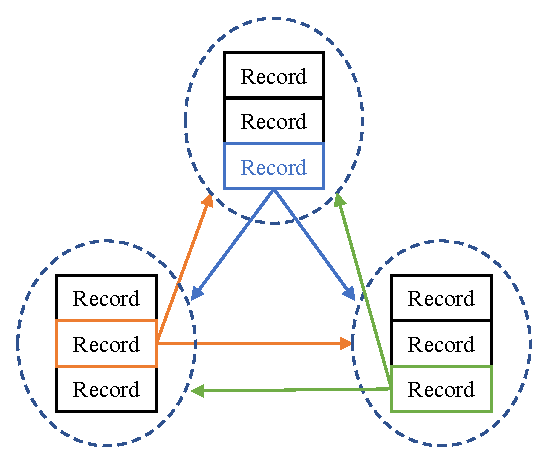
\includegraphics[width=.45\textwidth]{fig/ex.eps}}
\caption{A first-attempt approach.}
\label{fig:proto}
\end{figure}

\subsection{A First-Attempt Approach}
We designed our first system to demonstrate our basic ideas and expose possible bottlenecks of our design.
\subsubsection{Basic Protocol}
\paragraph{Data Structure.} Figure \ref{fig:ds} shows the data structure of each record. To ensure the data integrity, each record contains SHA256 sum of payload. The whole record is encrypted with the collector's public key to avoid malicious peers modify or steal data record.
\paragraph{Epoch.} For every epoch, each user only opens a small window period to accept other peers' data records. Epoch is defined by Internet time. Since anonymous data is collected in a low frequency in our scenario, a typical interval between each epoch will be several hours. We also require every user's local time to be close enough to the Internet time. Otherwise, it will not able to send or receive data.
\paragraph{Initialization.} A newly joined user does not have any data record received from other peers. Therefore, other peers can infer that data records sent by the newly joined user at the first epoch are all generated by itself. A user need to spend several epochs on warming-up before it can hide its identity. To avoid the first epoch problem, every user's data pool is initialized with fake data records, which can be filtered by the collector but cannot be recognized by other peers. With this mechanism, other peers cannot know whether the data records sent at the first epoch are generated by the newly joined user.
\paragraph{Broadcasting and Receiving.} Each epoch, a user randomly selects several data records from its data pool and broadcasts them to its peers. Meanwhile, the user also receives data records from its peers. The size of the data pool is limited, when the pool reaches its maximum size, the user will drop old records.
\paragraph{Collecting.} Each user maintains a connection to the collector by sending heartbeat packets. When the collector wants to retrieve the anonymous data back, it sends ``collect" signal with its signature to every node. After receiving the ``collect" signal, the user shuffles and submits the data pool to the collector.

\subsubsection{Limitations}
After testing the first-attempt approach, we found these limitations of our prototype:
\begin{enumerate}[label=(\roman*)]
    \item \textbf{Low average hop count.} Low hop count means the records have not been well-shuffled before submitting to the collector.
    
    \item \textbf{Not scalable.} When the user number increases, the collector's bandwidth usage grows several times higher than normal value. The user also faces buffer overflow problem in the large system.
    
    \item \textbf{Enumeration type attack.} Same record contents will generate exactly the same encrypted results. If the content is enumeration type, a malicious peer can infer clear text by comparing the record it received with encrypted results of possible values.
\end{enumerate}


\subsection{Improvements}
\paragraph{Data Record Duplication.} Information theory suggests that the entropy of a system is:
\begin{equation}
S=-\sum_{i=0}^n{P_i log_2 P_i}
\end{equation}
here $P_i$ is probability of event $i$, $n$ is the amount of all possible events. Sending a same record to several peers can decrease the value of each $P_i$ and increase $n$, which can increase the system's entropy. High entropy system means the records can be well shuffled.

\paragraph{Increasing Average Hop Count.} The cause of low average hop count is the probability of selecting a newly generated data record to send is low. To solve this issue, PEX divides the data pool into two separated queues, a hot queue and a cold queue. The hot queue prioritize data records with low hop count, which means newly generated records will be pushed into the hot queue. In addition, the hot queue's size is limited and all the sending records are selected from the hot queue. Therefore, data records with zero hop have higher priority to be selected to send. The cold queue has an unlimited size. It is used to store data records with high hop count. Since received data records at least have one hop, these data will be stored in the cold queue. When there are available slots in the hot queue, the user will randomly select some records with the lowest hop count from the cold queue and push them into the hot queue. Therefore, the hot queue is still obfuscated with other peers' data.

\paragraph{Salt.} If data record's contents are enumeration type, even the record is encrypted with collector's public key, other peers can still know the clear text. Because the encryption results of these enumeration typed data are deterministic. PEX adds a random salt section in front of payload to make sure two same records from different nodes have different encrypted results.

\section{Reducing Bandwidth Cost on Collector-Side}
Because of the duplication mechanism, the server will receive a same record for many times, causing huge waste on collector's bandwidth. To remove redundant records as many as possible, PEX divides the whole P2P network into many small groups. Each group has a group leader, who is responsible for collecting data from other group members and removing duplicated records. Then, the leader sends the data to the collector. Group leader is elected randomly each time the collector wants to retrieve data.

\subsection{Decentralized Voting Protocol}
Instead of using a centralized service to determine the group leader, PEX uses decentralized voting protocol to elect the leader. The protocol's safety is ensured by the hash function security. The decentralized voting protocol contains five stages:
\paragraph{\textit{Stage 1:} Random String Generation.} Each client generates a random string and calculate its SHA256 sum as the fingerprint. The string is long enough to resist brutal force search or rainbow table attack.
\paragraph{\textit{Stage 2:} Hash Value Broadcast.} Each client broadcasts its fingerprint to every peer in the group. Once every node received all other peers' fingerprint or a timeout situation occurred, the voting goes to its third stage.
\paragraph{\textit{Stage 3:} String Broadcast.} Each client broadcasts its random string to every peer in the group. Once every node received all other peers' random string or a timeout situation occurred, the voting goes to its fourth stage.
\paragraph{\textit{Stage 4:} Validation.} Each client checks whether random strings sent from other peers match its corresponding fingerprint. If no one sends a fraud string, the voting goes to its final stage.
\paragraph{\textit{Stage 5:} Election.} Each client sorts all random strings by using its fingerprint as the key. Next, the clients concatenate these strings and calculate its SHA256 sum. Last, modulo the SHA256 sum by the group size, and use the result as the index to find corresponding node as the group leader.

\subsection{Forming Voting Group\label{sec:form}}
To reach lowest duplication rate, a node should always try to join a group, and the group members should always try to include as more peers in the group as possible. Because the larger average group size, the fewer group leaders in the P2P network, which means data records will be more concentrated and leads to fewer duplication records.

When a node joins the P2P network, it searches for other available peers. The node queries the peer's group information and try to join its group. If the group is full or the node cannot connect to every other group member, the node will fail to join the group. Then, the node will try to establish a normal connection with the peer without joining its group, and then search for other groups to join.

However, according to one of the design principles in section \ref{sec:design}, a node should never reveal its peers information. If a node's peers all come the same group, then other group members will know the nodes' peer information, which obeys our design principle. To solve this problem, the peer limit should be greater than group size limit so that the node can also connect to peers outside of the group.

\subsection{Malicious Peer Protection}
In case of a group member intentionally breaks the voting rule to fight for the group leader, the decentralized voting protocol should provide mechanisms to ensure the election fairness.

\subsubsection{Silent Sender Attack}
If a node intentionally refuses to send its fingerprint or random string but still connected to group members, it will block the whole voting process. To prevent a single malicious node blocks the procedure, each stage has a timeout limit. When the node fails to receive fingerprints or strings from other peers before timeout, it will consider the peer who does not send the fingerprint or string in time gives up its voting right and broadcasts this event to other group members for synchronization.

\subsubsection{Last Sender Attack}
If the malicious node does not send the string and waits for other members to send their strings, then the node can construct a string which can make sure it can be elected as the group leader. However, other group members will not send their strings until they receive the fingerprint from this node. When the malicious node wants to send a specially constructed string, the other member already has its fingerprint. So, the constructed string must has the same fingerprint as the node sent in the previous stage to pass the validation stage. Under this strong constraint, it is almost impossible to find a string which can overturn the election result. The decentralized voting protocol is safe as long as the hash algorithm is safe.

\begin{figure}[h]
\centering
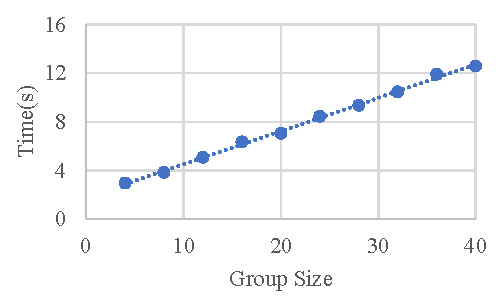
\includegraphics[width=.45\textwidth]{fig/latency.eps}
\caption{Decentralized voting latency, transportation latency between nodes are randomly selected between 10ms and 200ms.}
\label{fig:latency}
\end{figure}

\section{Evaluation}
To evaluate PEX, we implemented a simulator to simulates the behavior of the system. We measured system's voting performance, bandwidth usage, and duplication rate. We verified that PEX can 
\begin{enumerate*}[label=(\roman*)]
    \item perform decentralized voting with acceptable latency
    \item ensure most nodes belong to a full-sized group
    \item scale to as least 1 million users.
\end{enumerate*}

\subsection{Decentralized Voting Latency}
In the real world, most nodes typically have no more than 100 peers. So, we measured the voting performance in a small scale. Figure \ref{fig:latency} shows the decentralized voting latency. The latency grows linearly with the group size. Compared to the interval between data pulled from the collector is typically several hours or even several days, the voting latency is acceptable.

\subsection{Voting Group}
The number and the size of voting groups in a big network is strongly related to network's duplication rate. The fewer and larger the voting groups, the lower the duplication rate. If the average size of voting groups can maintain a value close to the group size limit while user number growing, it means the system has the potential to be scaled for real-world use.

Figure \ref{fig:avg_size} shows the average voting group size with respect to the number of users. The average group size reaches the limit rapidly and maintains a value close to the limit. Therefore, the number of group grows linearly, which is shown by figure \ref{fig:grp_cnt}.


\begin{figure*}[t]
\centering
\subfigure[Amount of voting groups - amount of users]{
\label{fig:grp_cnt}
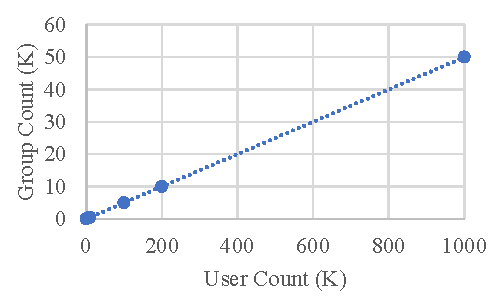
\includegraphics[width=.45\textwidth]{fig/gp_cnt.eps}}
\subfigure[Average group size - amount of users.]{
\label{fig:avg_size}
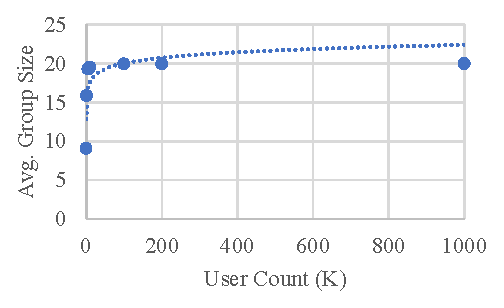
\includegraphics[width=.45\textwidth]{fig/avg.eps}}
\caption{Statistic data for group forming protocol. Probability of two nodes can be connected is 66.7\%, while the group size and number of peers is limited to 20 and 25, respectively.}
\label{fig:stat}
\end{figure*}

\begin{figure*}[t]
\centering
\subfigure[Records duplication rate - amount of users.]{
\label{fig:dup}
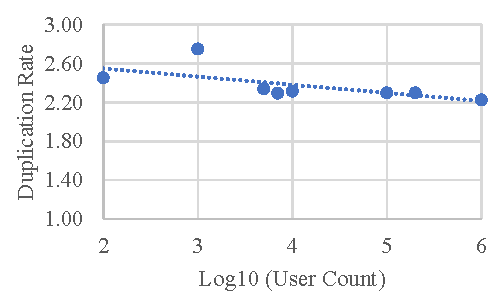
\includegraphics[width=.45\textwidth]{fig/dup.eps}}
\subfigure[Bandwidth saved - amount of users.]{
\label{fig:band}
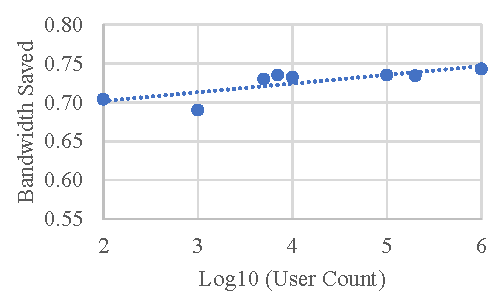
\includegraphics[width=.45\textwidth]{fig/band.eps}}
\caption{Simulation results after 100 epochs. Every node generates one record and randomly select 3 records then sends to 2 peers.}
\label{fig:scala}
\end{figure*}

\subsection{Bandwidth}
Figure \ref{fig:dup} shows the data duplication rate of the end-to-end simulation. Duplication rate does not grow when the number of users increases. It proves that the collector's bandwidth complexity is $O(n)$. Compared to traditional anonymous data collection system that every client sends its own records to the collector, whose bandwidth complexity is also $O(n)$, PEX has a reasonable bandwidth cost.

Figure \ref{fig:band} shows the bandwidth saved by dividing network into small voting groups. Compared to our first-attempt approach, PEX saves up to 75\% bandwidth cost.

PEX's end-to-end performance shows that it is well-designed for horizontal-scalability. PEX can support up to 1 million users, providing metadata protection with an acceptable bandwidth overhead.

\section{Conclusion and Future Work}
We designed and implemented a peer-to-peer based anonymous data collection system called PEX. PEX shuffles data records in a peer-to-peer network. Each user randomly selects some records from its pool and send their replicas to several peers. To reduce the collector's bandwidth burden, records are de-duplicated in small local groups before sending to the collector's servers. Our simulation shows PEX can save bandwidth up to 75\% compared to our baseline result. PEX is scalable to millions of users demonstrated in out simulation results.

This work leaves some possible future works, including:
\begin{enumerate*}[label=(\roman*)]
    \item theoretical proof of resilience to traffic-pattern attack
    \item design new mechanisms to reduce the duplication rate
    \item design a more efficient decentralized voting protocol.
\end{enumerate*}

{\footnotesize 
\bibliographystyle{acm2}
\bibliography{references.bib}}

\end{document}
